\section{Calibration, thresholds and the sheep failure}
\label{sec:supp_calibration}
\paragraph{Per-image thresholds.}
If the hierarchy's gain is calibration, could a per-image threshold computed from each map recover it, or repair sheep? We tested seven rules on the counts and stored maps of the main run. Each rule's $\tau_I$ is snapped to the 17-point grid, so the existing counts score it exactly, raw and with DenseCRF (the stored maps reproduce the counted mask areas with Pearson $\ge0.9998$). The rules are: T0, the global threshold; T1, Otsu; T2, the crossing of a two-Gaussian fit; T3, $\mu_I+k\sigma_I$; T4, the most stable threshold (smallest area change); T5, the capped map's ranking at the fine-only map's area; and T6, Otsu plus an offset. One-parameter rules choose their parameter inside the training folds. The rule set was registered before the run. Table~\ref{tab:supp_threshold} gives the outcome. No rule improves the capped pipeline. Matching the fine-only map's area (T5) repairs sheep ($-0.007$ instead of $-0.092$) but gives back most of the gain. Otsu helps the fine-only map in four folds but loses 0.021 on COCO-Cap. Two-Gaussian and $\mu{+}k\sigma$ thresholds often fall outside the grid (20--87\% of images).

\begin{table}[t]
\centering
\footnotesize\setlength{\tabcolsep}{2.6pt}
\begin{tabular}{@{}llcccc@{}}
\toprule
Map (+ DenseCRF) & Rule & VOC OOF & vs.\ same map T0 & sheep $\Delta$ & COCO \\
\midrule
fine only & T0 global & .8230 & -- & -- & .6623 \\
fine only & T1 Otsu & .8283 & +.0054 (4/5) & $-$.041 & .6411 \\
fine only & T4 stable & .8255 & +.0026 (2/5) & $-$.042 & .6809 \\
fine only & T6 Otsu$+d$ & .8276 & +.0046 (3/5) & $-$.041 & .6411 \\
\midrule
C2F + cap & T0 global & \textbf{.8293} & -- & $-$.092 & \textbf{.6964} \\
C2F + cap & T1 Otsu & .8238 & $-$.0055 (1/5) & $-$.079 & .6359 \\
C2F + cap & T2 two-Gauss. & .8031 & $-$.0262 (0/5) & $-$.080 & .6258 \\
C2F + cap & T3 $\mu{+}k\sigma$ & .7864 & $-$.0429 (0/5) & $-$.254 & .6498 \\
C2F + cap & T4 stable & .8239 & $-$.0054 (1/5) & $-$.108 & .6722 \\
C2F + cap & T5 fine-only area & .8246 & $-$.0047 (0/5) & $-$.007 & .6659 \\
C2F + cap & T6 Otsu$+d$ & .8297 & +.0004 (2/5) & $-$.090 & .6586 \\
\bottomrule
\end{tabular}
\caption{\textbf{Per-image threshold rules} (after DenseCRF; sheep $\Delta$ vs.\ fine-only T0). Both registered selectors kept the fine-only global threshold. Per-image oracle (best grid threshold per image, using ground truth): 0.896 fine-only vs.\ 0.895 C2F + cap on VOC-Sim.}
\label{tab:supp_threshold}
\end{table}

\paragraph{Sheep.}
The sheep loss is a loss of recall: 294{,}665 fewer true-positive pixels, against only 12{,}173 more false positives. It is concentrated in close-ups where the sheep covers 79--96\% of the frame. Figure~\ref{fig:supp_sheep} shows that the capped map is better on sheep at every threshold above 0.45. Below that, its false positives are twice those of the fine-only map, so sheep cannot use the low threshold it prefers. Across all classes, objects that fill more than 75\% of the frame gain from the cap at every threshold. Sheep is the exception because its surroundings are grouped with it at low thresholds. Figure~\ref{fig:supp_sheep_case} shows the median sheep image.

\begin{figure}[t]
\centering
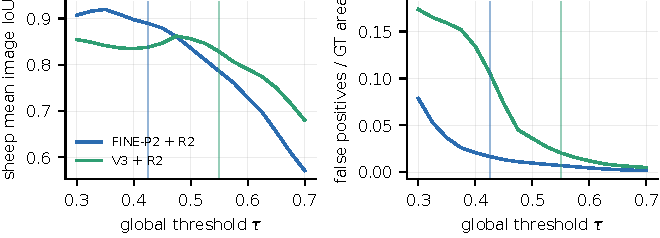
\includegraphics[width=\columnwidth]{figures/supp_sheep_curves.pdf}
\caption{\textbf{Sheep across thresholds} (25 VOC-Sim images, after DenseCRF). Vertical lines: the global thresholds of the two pipelines.}
\label{fig:supp_sheep}
\end{figure}

\begin{figure}[t]
\centering
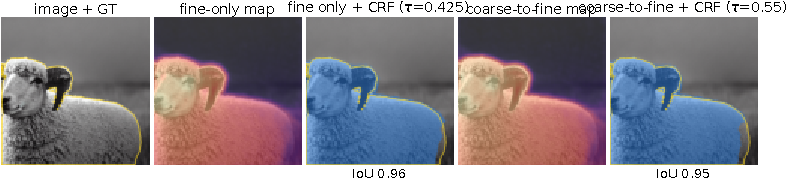
\includegraphics[width=\columnwidth]{figures/supp_sheep_case.pdf}
\caption{\textbf{The median sheep image} (median change of the capped pipeline against fine-only, both after DenseCRF, at their global thresholds).}
\label{fig:supp_sheep_case}
\end{figure}
\clearpage
